\documentclass[]{book}
\usepackage{lmodern}
\usepackage{amssymb,amsmath}
\usepackage{ifxetex,ifluatex}
\usepackage{fixltx2e} % provides \textsubscript
\ifnum 0\ifxetex 1\fi\ifluatex 1\fi=0 % if pdftex
  \usepackage[T1]{fontenc}
  \usepackage[utf8]{inputenc}
\else % if luatex or xelatex
  \ifxetex
    \usepackage{mathspec}
  \else
    \usepackage{fontspec}
  \fi
  \defaultfontfeatures{Ligatures=TeX,Scale=MatchLowercase}
\fi
% use upquote if available, for straight quotes in verbatim environments
\IfFileExists{upquote.sty}{\usepackage{upquote}}{}
% use microtype if available
\IfFileExists{microtype.sty}{%
\usepackage{microtype}
\UseMicrotypeSet[protrusion]{basicmath} % disable protrusion for tt fonts
}{}
\usepackage{hyperref}
\hypersetup{unicode=true,
            pdftitle={Application for Tenure-Track Instructor Position in Statistics at UBC},
            pdfauthor={Vincenzo Coia},
            pdfborder={0 0 0},
            breaklinks=true}
\urlstyle{same}  % don't use monospace font for urls
\usepackage{natbib}
\bibliographystyle{apalike}
\usepackage{longtable,booktabs}
\usepackage{graphicx,grffile}
\makeatletter
\def\maxwidth{\ifdim\Gin@nat@width>\linewidth\linewidth\else\Gin@nat@width\fi}
\def\maxheight{\ifdim\Gin@nat@height>\textheight\textheight\else\Gin@nat@height\fi}
\makeatother
% Scale images if necessary, so that they will not overflow the page
% margins by default, and it is still possible to overwrite the defaults
% using explicit options in \includegraphics[width, height, ...]{}
\setkeys{Gin}{width=\maxwidth,height=\maxheight,keepaspectratio}
\IfFileExists{parskip.sty}{%
\usepackage{parskip}
}{% else
\setlength{\parindent}{0pt}
\setlength{\parskip}{6pt plus 2pt minus 1pt}
}
\setlength{\emergencystretch}{3em}  % prevent overfull lines
\providecommand{\tightlist}{%
  \setlength{\itemsep}{0pt}\setlength{\parskip}{0pt}}
\setcounter{secnumdepth}{5}
% Redefines (sub)paragraphs to behave more like sections
\ifx\paragraph\undefined\else
\let\oldparagraph\paragraph
\renewcommand{\paragraph}[1]{\oldparagraph{#1}\mbox{}}
\fi
\ifx\subparagraph\undefined\else
\let\oldsubparagraph\subparagraph
\renewcommand{\subparagraph}[1]{\oldsubparagraph{#1}\mbox{}}
\fi

%%% Use protect on footnotes to avoid problems with footnotes in titles
\let\rmarkdownfootnote\footnote%
\def\footnote{\protect\rmarkdownfootnote}

%%% Change title format to be more compact
\usepackage{titling}

% Create subtitle command for use in maketitle
\providecommand{\subtitle}[1]{
  \posttitle{
    \begin{center}\large#1\end{center}
    }
}

\setlength{\droptitle}{-2em}

  \title{Application for Tenure-Track Instructor Position in Statistics at UBC}
    \pretitle{\vspace{\droptitle}\centering\huge}
  \posttitle{\par}
    \author{Vincenzo Coia}
    \preauthor{\centering\large\emph}
  \postauthor{\par}
      \predate{\centering\large\emph}
  \postdate{\par}
    \date{2019-12-10}


\begin{document}
\maketitle

{
\setcounter{tocdepth}{1}
\tableofcontents
}
\hypertarget{cover-letter}{%
\chapter{Cover Letter}\label{cover-letter}}

\textbf{NOTE: THIS APPLICATION IS A WORK-IN-PROGRESS}

Cover letter STATUS:

\begin{itemize}
\tightlist
\item[$\square$]
  Brain dump of ideas
\item[$\square$]
  Organization of ideas
\item[$\square$]
  Filling in gaps
\item[$\square$]
  Smooth over to form a draft
\item[$\square$]
  Complete: no changes needed.
\end{itemize}

Dear members of the search committee,

I am writing to enthusiastically apply for a tenure-track instructor position in Statistics (\href{https://www.stat.ubc.ca/three-tenure-track-instructor-positions-statistics-35876}{Job \#35876}). Ever since joining the department of Statistics full time in early 2017 to advance our Data Science initiatives, I've come to realize just how ideal of a fit the educational leadership stream is for me. My aim with this application is to indicate why this is so, as well as why the department and UBC (and external to UBC!) would benefit by promoting me to the educational leadership stream.

Ultimately, in this position, I envision advancing all branches of Data Science education at UBC, especially through Statistics for Data Science. I'm equally excited to develop the new Minor in Data Science program as I am to continue developing the Master of Data Science (MDS) program. In fact, I'm actually rather torn between the two: there is still much to develop with MDS, and I'm rather invested in the program; but the allure of developing a new Minor program is a new equally exciting challenge that I can make valuable contributions to. Regardless of my level of involvement in these, I intend to keep an open stream of communication between the two programs, along with STAT 545A/547M, so that data science education at UBC can overall grow as a cohesive whole, as opposed to competing pieces.

My vision for doing this

I've identified four pillars of my career, which I hope will lay the foundation for my vision going forward in the teaching stream, as well as convey fit on my end. They are, in order of culmination:

\begin{enumerate}
\def\labelenumi{\arabic{enumi}.}
\item
  \textbf{Application}: addressing real problems with data science.
\item
  \textbf{Research}: discovering better ways to do data science.
\item
  \textbf{Development}: turning new research into programs and tools, which are ideally accessible to the public.
\item
  \textbf{Teaching}: spreading data literacy and enthusiasm to the public.
\end{enumerate}

Lastly, I'd like to elaborate on how my skills will be an asset to the department.

Excitement and promise for starting up the minor program, helping MDS and STAT 545A/547M evolve along with it.

hyperlinks to one or two examples of my teaching materials. Note that I don't see any of these as being ``finished'', but rather a work-in-progress.

\begin{itemize}
\tightlist
\item
  For STAT 545A/547M (Exploratory Data Analysis), I made the \href{https://stat545guidebook.netlify.com/}{lecture notes} and \href{https://stat545.stat.ubc.ca/}{course website}. Less relevant are Lectures 11+, taught by Dr.~Firas Moosvi, and Lecture 6, a guest lecture taught by my TA, Victor Yuan.
\item
  For DSCI 551 (Probability for Data Science), I wrote the \href{https://ubc-mds.github.io/DSCI_551_stat-prob-dsci/lectures/}{lecture notes} by using Dr.~Mike Gelbart's notes from the previous year as scaffolding.
\item
  I'm writing an open-source book on regression analysis for data science, called \href{https://interpreting-regression.netlify.com/}{Interpreting Regression}. It's in its early stages.
\end{itemize}

What I'm comfortable teaching (useful in parallel to the minor program in DS)

Tools; my comfort level with CS. Although I don't have formal training in CS outside of perhaps a few undergraduate courses, my approach to learning these things is to identify tools and techniques that would be useful, and commit to building these tools. I prefer this approach over prescribed training such as online courses, because I find it more genuine as I encounter concepts as they become relevant. For example, I've been learning web hosting as I've been learning about Hugo, blogdown, and netlify to create websites like my homepage, course websites like STAT 545A/547M, and hosting ``books'' such as Interpreting Regression online. I've learned shell scripting back in my PhD, and continue to learn more, as I embrace GNU Make and workflow automation in general.

Teaching tools and methods

In this application, I'll show you how my career goals are related to teaching and educational leadership. You'll read about my plans to continue reframing statistics for the purpose of data science by writing books such as interpreting regression and writing software such as dist fire.

the names of three references who have been asked to send reference letters:

\begin{enumerate}
\def\labelenumi{\arabic{enumi}.}
\tightlist
\item
  Dr.~Tiffany Timbers (current supervisor)
\item
  Dr.~Michael Gelbart (current supervisor)
\item
  Dr.~Harry Joe (PhD supervisor)
\end{enumerate}

I am eager to begin the position on the indicated July 1, 2020 start date, but am ultimately flexible.

Enthusiastically yours,

Dr.~Vincenzo Coia

\hypertarget{curriculum-vitae}{%
\chapter{Curriculum Vitae}\label{curriculum-vitae}}

\hypertarget{work-experience}{%
\section{Work Experience}\label{work-experience}}

2017/01 - present\\
\textbf{Lecturer of Data Science}\\
(Initially: Postdoctoral Teaching and Learning Fellow)\\
Masters of Data Science Program, and the Department of Statistics\\
The University of British Columbia\\
Vancouver, BC

2009/05 - 2014/05\\
\textbf{Short-term statistical consulting} (6 projects)\\
UBC and private

\hypertarget{education}{%
\section{Education}\label{education}}

\textbf{PhD in Statistics}\\
2012/09 - 2017/02\\
The University of British Columbia\\
Conferred May 29, 2017

\textbf{MSc in Mathematics and Statistics (Statistics)}\\
2011/09 - 2012/08\\
Brock University\\
Conferred on October 13, 2012

\textbf{BSc (3-year) in Biological Sciences}\\
Minor in Earth Sciences\\
2005/09 - 2011/04\\
Brock University\\
Conferred ``With Distinction'' on October 22, 2011

\textbf{BSc (Honours) Mathematics Integrated with Computers and Applications}\\
Concentration in Statistics\\
2005/09 - 2011/04\\
Brock University\\
Conferred ``With First-Class Standing'' on June 7, 2011

\hypertarget{volunteer-positions}{%
\subsection{Volunteer Positions}\label{volunteer-positions}}

2016/09 - 2016/02\\
\textbf{Science World at TELUS World of Science }\\
Vancouver, BC\\
78.15 hours

2013/10 - 2014/05\\
\textbf{Beaty Biodiversity Museum: Events Volunteer}\\
Vancouver, BC\\
35.0 hours

2013/04 - 2013/09\\
\textbf{UBC Farm}\\
Vancouver, BC\\
102.5 hours

2011/06 - 2011/08\\
\textbf{Project S.H.A.R.E. community garden}\\
Niagara Falls, ON\\
15.0 hours

\hypertarget{research-assistantships}{%
\subsection{Research Assistantships}\label{research-assistantships}}

2013/05 - 2013/08\\
\textbf{Robust penalized regression}\\
Supervisor: Dr.~Gabriela Cohen-Freue\\
Department of Statistics\\
The University of British Columbia\\
Vancouver, BC

2012/05 - 2012/08\\
2011/05 - 2011/08\\
2010/05 - 2010/08\\
\textbf{Extreme value modelling}\\
Supervisor: Dr.~Mei Ling Huang\\
Department of Mathematics\\
Brock University\\
St.~Catharines, ON

2010/09 - 2011/06\\
\textbf{Quantum monte carlo simulations}\\
Supervisors: Dr.~Stuart Rothstein; Dr.~Wai Kong (John) Yuen\\
Department of Chemistry and Department of Mathematics\\
Brock University\\
St.~Catharines, ON

\hypertarget{teaching-assistantships}{%
\subsection{Teaching Assistantships}\label{teaching-assistantships}}

\textbf{Duration}: From the latter part of my undergrad, to the end of my PhD.

UBC:

\begin{itemize}
\tightlist
\item
  \textbf{SCIE 300: Communicating Science} (5x)
\end{itemize}

Brock University:

\begin{itemize}
\tightlist
\item
  \textbf{MATH 4P82/5P82: Non-parametric Statistics}
\item
  \textbf{MATH 3P82: Regression Analysis}
\item
  \textbf{MATH 4P81/5P81: Sampling Theory}
\item
  \textbf{MATH 3P81: Experimental Design} (2x)
\item
  \textbf{MATH 2F40: Mathematics Integrated w/ Computers and Applications II}
\end{itemize}

\hypertarget{publications-and-talks}{%
\section{Publications and Talks}\label{publications-and-talks}}

\hypertarget{articles-submitted-to-refereed-journals}{%
\subsection{Articles Submitted to Refereed Journals}\label{articles-submitted-to-refereed-journals}}

\begin{itemize}
\item
  Huang, M.L., Coia, V., and Brill, P.H. (2013) A cluster truncated
  Pareto distribution and its applications. ISRN Probability and
  Statistics 2013: Article ID 265373.
\item
  Ayad, M., Coia, V., and Kihel, O. (2014) The number of relatively
  prime subsets of a finite union of sets of consecutive integers.
  Journal of Integer Sequences 17: Article 14.3.7
\item
  Coia, V., and Huang, M.L. (2014) A sieve model for extreme
  values. Journal of Statistical Computation and Simulation.
  84(8):16921710.
\end{itemize}

\hypertarget{articles-submitted-to-conference-proceedings}{%
\subsection{Articles Submitted to Conference Proceedings}\label{articles-submitted-to-conference-proceedings}}

\begin{itemize}
\tightlist
\item
  Huang, M. L., Coia, V., and Brill, P.H., A mixture truncated
  Pareto distribution, In JSM Proceedings 2012, Statistical Computing
  Section, Alexandria, VA: American Statistical Association, pp.

  \begin{enumerate}
  \def\labelenumi{\arabic{enumi}.}
  \setcounter{enumi}{24882497}
  \item
  \end{enumerate}
\end{itemize}

\hypertarget{conference-and-roundtable-contributions}{%
\subsection{Conference and Roundtable Contributions}\label{conference-and-roundtable-contributions}}

\begin{itemize}
\item
  Coia, V., Nolde, N., and Joe, H. Forecasting Extremes for Flooding
  (Invited Talk). The 44th Annual Meeting of the Statistical Society
  of Canada. May 29June 1, 2016 at Brock University, St.~Catharines,
  ON.
\item
  Coia, V., and Jeanniard du Dot, T. (Invited Demonstration) ``Using
  the Grammar of Graphics and Interactivity to explore Biologging Data
  in R''. May 6, 2015. Building a Bioanalytical Theory for Analysis of
  Marine Mammal Movements: A Peter Wall International Research
  Roundtable. The University of British Columbia, Vancouver, BC.
\item
  Coia, V. ``Flood Warning: An Application of High-Quantile Regression''
  (Contributed Talk). SFU/UBC Joint Graduate Student Seminar (Winter).
  February 28, 2015 at the SFU Harbour Centre, Vancouver, BC.
\item
  Coia, V. ``A New Sieve Model for Extreme Values'' (Contributed Talk).
  SFU/UBC Joint Graduate Student Seminar (Fall). September 29, 2012 at
  the SFU Harbour Centre, Vancouver, BC.
\item
  Coia, V., and Huang, M.L. ``On Estimation of Heavy Tailed
  Distributions'' (Contributed Talk). The 40th Annual Meeting of the
  Statistical Society of Canada. June 36, 2012 at the University of
  Guelph, Guelph, ON.
\item
  Huang, M.L., Coia, V., and Brill, P.H. ``A Mixture Truncated Pareto
  Distribution'' (Contributed Talk). The 2012 Joint Statistical
  Meetings. July 28August 2, 2012 at San Diego, California
\end{itemize}

\hypertarget{awards}{%
\section{Awards}\label{awards}}

\hypertarget{university-issued}{%
\subsection{University Issued}\label{university-issued}}

\begin{itemize}
\tightlist
\item
  2012/09 - 2016/08: Four-Year Fellowship
\item
  2012/09 - 2016/08: Faculty of Science Graduate Award
\item
  2011/09: Dean of Graduate Studies Excellence Scholarship
\item
  2011/06/07: Dean's Gold Medal
\item
  2011/06/07: Distinguished Undergraduate Student Award in Mathematics
\item
  2011/03: President's Surgite Award
\end{itemize}

\hypertarget{nationally-recognized}{%
\subsection{Nationally Recognized}\label{nationally-recognized}}

\begin{itemize}
\tightlist
\item
  2013/06: Governor General of Canada's Gold Medal
\item
  2012/09 - 2015/08: NSERC Postgraduate Award (Doctoral, 3-year)
\item
  2011/09 - 2012/08: NSERC Alexander Graham Bell Canada Graduate Scholarship (Masters)
\item
  2010/05 - 2010/08: NSERC Undergraduate Student Research Award
\end{itemize}

\hypertarget{individual-donors}{%
\subsection{Individual Donors}\label{individual-donors}}

\begin{itemize}
\tightlist
\item
  2012/04: Dr.~Jack Lightstone \& Dorothy Markiewicz Scholarship
\item
  2012/04: Dr.~Raymond \& Mrs.~Sachi Moriyama Grad. Fellowship
\item
  2012/03: Tomlinson Entrance Scholarship for Excellence in Mathematics and Science
\item
  2011/06: John and Roslyn Reed Book Prize
\item
  2010/09: Art Bicknell Scholarship in Mathematics
\item
  2010/09: Ian D. Beddis Family Scholarship
\item
  2010/09: Terry and Sue White Mathematics and Science Scholarship
\item
  2007/09: M.J. (``Mel'') Farquharson Scholarship
\item
  2006/09: Scholler Foundation Scholarship in Chemistry
\end{itemize}

\hypertarget{athletic-awards}{%
\subsection{Athletic Awards}\label{athletic-awards}}

\begin{itemize}
\tightlist
\item
  2016/04/03: Sportsmanship Award, UBC Thunderbirds Sport Clubs (Fencing)
\item
  2016/02/28: Bronze Medal in Senior Mixed Epee (Intercollegiate Tournament, UBC)
\item
  2015/11/16: Bronze Medal in Senior Mixed Epee (Remembrance Day Tournament, UBC)
\item
  2012/03/28: RM Davis Surgite Award
\item
  2009/12/12: First Place Award Winter Epeedemic, Toronto Fencing Club
\item
  2009/03: Varsity Fencing Rookie of the Year Award
\end{itemize}

\hypertarget{declined-awards}{%
\subsection{Declined Awards}\label{declined-awards}}

\begin{itemize}
\tightlist
\item
  2012/04: Ontario Graduate Scholarship (Doctoral)
\item
  2011/05: Ontario Graduate Scholarship (Masters)
\end{itemize}

\hypertarget{professional-activities}{%
\section{Professional Activities}\label{professional-activities}}

Dept. of Statistics, The University of British Columbia:

\begin{itemize}
\tightlist
\item
  2016/05 - 2016/06: \textbf{Search committee member (for CRC 2 faculty position)}
\item
  2015/04/30: \textbf{Organizer of the ``\href{http://stat.ubc.ca/~vincen.coia/abstractworkshop.html}{How to Write an Awesome Abstract}'' workshop}
\item
  2014/06 - 2015/05: \textbf{Organizer of the \href{http://stat.ubc.ca/~vincen.coia/seminar.html}{SFU/UBC Joint Seminar}}
\item
  2014/06 - 2014/09: \textbf{Organizer of the Graduate Student Trip}
\item
  2014/04 - 2015/05: \textbf{Co-founder of the Graduate Writing Forums}
\item
  2013/06 - 2014/05: \textbf{Statistics Graduate Student Representative}
\end{itemize}

\hypertarget{statement-of-vision-for-education-in-statistics-and-data-science}{%
\chapter{Statement of vision for education in statistics and data science}\label{statement-of-vision-for-education-in-statistics-and-data-science}}

STATUS:

\begin{itemize}
\tightlist
\item[$\boxtimes$]
  Brain dump of ideas
\item[$\boxtimes$]
  Organization of ideas
\item[$\boxtimes$]
  Filling in gaps
\item[$\square$]
  Smooth over to form a draft
\item[$\square$]
  Complete: no changes needed.
\end{itemize}

My vision for EL involves:

\begin{itemize}
\tightlist
\item
  reframing the map of statistics from the perspective of data science to provide a framework for solving real-world problems
\item
  bringing to life underutilized tools and techniques.
\item
  Stewardship of data science: defining data science and maintaining a vision for our organizations (minor program; MDS; STAT 545A/547M, etc), promoting responsible use of data science.
\end{itemize}

Why does the way in which we approach statistics for data science need reframing? In short, this is because Statistical Science focusses on describing consequences of a framework of stochastic assumptions (a ``framework-first'' approach), and Data Science focusses on addressing real-world problems using tools described by Statistical Science (a ``problem-first'' approach). The ability to solve real-world problems does not directly follow from Statistical Science, because real problems don't neatly satisfy assumptions. Instead, Statistics for Data Science involves a critical evaluation of assumptions in terms of their usefulness and their goodness of approximation -- this is more than ``assumption checking'', it's ``assumption building''. Even Applied Statistics may seem to take a problem-first approach, but the motivating real-world problem tends to be used as motivation for setting up a framework of assumptions, for which properties are then described (as usual).

Reframing Statistics for Data Science involves modularizing \emph{scenarios} instead of \emph{methods}. Perhaps the best example of this is DSCI 562 (Regression II), which I re-developed last year. Instead of teaching ``GLM's'' and ``Survival Analysis'', I teach ``Regression when the range of the response is restricted'', or ``Regression when data are censored''. The idea behind this is that students can then handle combined scenarios, such as ``regression when the range of the response is restricted and data are censored'', because they've learned model \emph{modifications} in each topic, not just the isolated models themselves. This scenario-first approach naturally promotes motivation in the classroom, because the topics are designed to be practical. This is also a tremendous opportunity for me and UBC, because I'm finding a general lack of this type of focus. I'm hoping to be a leader in this area. Because I take a scenario-based approach, it's important to find motivating real-world problems to lead a powerful discussion. Where possible, I draw from my industry experience and capstone. For example, using the BCMEA example for DSCI 551, flood forecasting for DSCI 562, or determining the effect of blue-light-blocking glasses on sleep for DSCI 561. I've found that these examples spur lots of great discussion.

To reframe Statistics, I've been developing a book called ``Interpreting Regression'' that teaches a scenario-first approach, and intent to continue its development. When I've had the opportunity, I've been writing course notes to be recycled in this book. Some of the topics which I feel have a new perspective include:

\begin{itemize}
\tightlist
\item
  Survival analysis resources focus on the how of the Proportional hazards or Accelerated Failure models, or the survival curve estimation. First of all, with a lack of attention placed on the value and interpretation of distributions, survival curves and hazard functions are right off the bat a confusing introduction. Then, why we would even bother estimating such a thing, or setting up such a model, are not discussed. Also, the relationship between the Kaplan-Meier survival curve and the survival regression models is not clear. It's also not clear how one would apply machine learning methods with censored data. Again -- the framework has been set up (assumptions laid out for PH model or AF model), and properties described of these models (beta's are log hazard ratio), but this leaves students thinking ``I guess this is just what we do when faced with censored data'', as opposed to the more creative approach of making decisions on the modular components of modelling.
\item
  The teaching of MLE focusses on the how, and even then, it's hard to find a good resource on the how. But, after ample searching, I've yet to find the why of MLE, and this is because it's not framed in terms of deciding which assumptions to enforce in your model.
\item
  multiple imputation for missing data as plugging in a distribution to get marginal quantities. Without this being explained, students are left thinking ``I guess we should just use multiple imputation when faced with missing data, because that's just what we do''.
\end{itemize}

With a reframing of Statistics brings to light areas of Statistics that are useful, yet are not receiving much attention. These underutilized tools and techniques have already been described by statisticians, but their underuse perhaps stems from their misunderstanding / emphasis as only being required as assumptions, as well as our community's obsession with the mean. In addition to writing about these, I'm also developing software. Here are examples:

\begin{itemize}
\tightlist
\item
  There is a wealth of value that using both parametric and non-parametric distributions for the response can bring to data science -- ``distributional forecasting''.

  \begin{itemize}
  \tightlist
  \item
    I am developing an R package that works with distributions as objects, as opposed to handling the unwieldly pieces of functions like \texttt{dnorm()} and \texttt{rnbinom()}. My goal is to submit this package to CRAN and ROpenSci, and perhaps grab the attention of RStudio and the \texttt{tidymodels} team.
  \end{itemize}
\item
  By extension, another area of statistics that I believe are underappreciated are copulas. Once distributional forecasting is truly appreciated, then copulas become invaluable for parametric modelling for prediction, as well as providing new insight into the properties of data. I believe that copulas are currently not accessible enough due to complicated formulas and jargon, yet are tremendously useful for distributional forecasting. I hope to make this framework more accessible by developing an R package called \texttt{coperate} and \texttt{cmc} for easy manipulation of copulas, and easily created copula-based models (respectively).
\item
  Extreme value modelling also becomes invaluable for those cases that have heavy tailed data, such as at least one capstone project from Seahorse strategies (the team didn't end up using EVT because of lack of attention here, but should have), as well as organizations tackling the issue of flood forecasting and flood frequency assessments. Again, submitted to CRAN and ROpenSci. Extreme value models will be easy to build using the distplyr package I mentioned earlier by easily grafting distributional tails with \texttt{distplyr::right\_connect()} and \texttt{distplyr::left\_connect()}.
\end{itemize}

I also envision being a steward for data science by defining data science and hosting a data science workshop / conference. This is important to keep the dialogue open about just how we should go about teaching data science (so that insight such as what's presented here is spread), and what we should consider as being within the realm of data science. Taking the opportunity early to do this will help in our efforts of establishing ourselves as leaders in the field of data science. The beginnings of this workshop are underway, the first step of which was defining a vision for MDS, which I initiated.

I envision using the above three components for developing curricula at UBC, whether it be comtinuing to develop MDS, building a minor program, or other things. I also envision making this material public to establish ourselves as leaders in data science. Examples of courses that I've already redeveloped:

\begin{itemize}
\tightlist
\item
  Curriculum development of 551 throughout the years; 561 w/ Gaby and Sunny, later Tom; 531; 511?; 563; BAIT 509; 562; STAT 545A/547M (expanded Jenny's work, but this needs more help, especially in the face of a changing data science landscape at UBC).
\end{itemize}

\begin{figure}
\centering
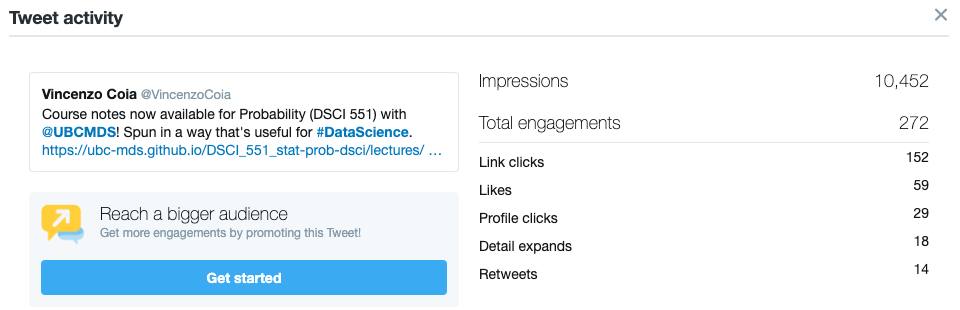
\includegraphics{./img/551_tweet.png}
\caption{DSCI 551 tweet activity}
\end{figure}

Lastly, an area that is crucial for EL, yet might not be called EL itself, is continuing to work with external partners, such as the Master of Data Science (MDS) capstone partners, to understand their pressing data issues, and lend a hand once in a while. As Stephen Covey says in ``The 7 Habits of Highly Effective People'', to be effective, one must ``sharpen the saw'' to keep yourself healthy -- except here, this is about remaining current and relevant. This is important for keeping myself and data science education at UBC relevant, as well as continually expanding my skillset. Besides having mentored MDS capstone projects for the past three years, I also did some work on flood forecasting with BGC Engineering this past summer, and plan to continue doing more. There are also simpler ways to sharpen the saw, including staying in touch with the data science community through Twitter, students and colleagues at UBC, newsletters such as ROpenSci and RStudio, as well as just plain looking for solutions to a new problem, or new solutions to an old problem.

To summarize my envisioned educational leadership throughout my career, as I see it now:

\begin{itemize}
\tightlist
\item
  Developing R packages with colleagues to help reframe statistics for data science through modular assumptions:

  \begin{itemize}
  \tightlist
  \item
    distplyr for distributional forecasting: distributions as S3 objects in R, which can be manipulated and easily visualized.
  \item
    coperate for easily understanding and handling copulas.
  \item
    cmc
  \end{itemize}
\item
  Writing public resources. I envision these as being ``go-to'' resources for learning, and making decisions based on the modularity of assumptions.

  \begin{itemize}
  \tightlist
  \item
    Books for reframing statistics, starting with ``Interpreting Regression'', then perhaps moving on to distributional forecasting.
  \item
    Vignettes and journal articles about the use of said R packages.
  \item
    Course materials made public.
  \item
    Data science ``cheat sheets'', especially when it comes to a guide for making decision about model assumptions.
  \end{itemize}
\item
  Hosting an annual ``Education in Data Science'' workshop/conference (we are already in the early stages of this).

  \begin{itemize}
  \tightlist
  \item
    Also, keeping an MDS vision statement.
  \end{itemize}
\end{itemize}

``Sharpening the saw'' by work with other organizations, and keeping up with the community.

\hypertarget{statement-of-teaching-and-training-philosophy}{%
\chapter{statement of teaching and training philosophy}\label{statement-of-teaching-and-training-philosophy}}

\hypertarget{teaching-philosophy}{%
\section{Teaching Philosophy}\label{teaching-philosophy}}

STATUS:

\begin{itemize}
\tightlist
\item[$\boxtimes$]
  Brain dump of ideas
\item[$\boxtimes$]
  Organization of ideas
\item[$\boxtimes$]
  Filling in gaps
\item[$\boxtimes$]
  Smooth over to form a draft
\item[$\square$]
  Complete: no changes needed.
\end{itemize}

My philosophy on teaching can best be broken down into four categories: \textbf{appropriate course structure}, \textbf{responsive teaching}, \textbf{motivation}, and \textbf{self-improvement}.

\hypertarget{appropriate-structure}{%
\subsection{Appropriate Structure}\label{appropriate-structure}}

You and I don't really know English. We only know enough for it to be a sufficiently useful tool for our own daily activities. I take this concept to heart as I design and deliver my courses. It's fallacious to design a course around \emph{topics}, but rather on building \emph{skills} for a certain purpose. To me, these skills formulated as a list of \textbf{learning objectives} (LO's) act as a ``true north'' that all components of a course point towards, and are the most important structure to the course. For example, course content on the topic ``heteroskedasticity'' could be developed in many directions. The students, thinking they have to ``know heteroskedasticity'', get stuck studying its never-ending scope. Instead, a learning objective such as ``modify a linear model to appropriately incorporate heteroskedasticity based on data diagnostics'' provides direction for the teaching team to create material, and clarity for the students. For concrete examples, take a look at \href{https://ubc-mds.github.io/DSCI_551_stat-prob-dsci/lectures/}{the DSCI 551 notes}, or my other course materials.

Clarity about the course structure and expectations is important for equipping students with a map of what they need to do to succeed. In addition to discussing how students should use the LO's, describing the summative assessments and a course syllabus is also important, as well as making it easy to navigate course material (see, for example, the \href{https://stat545.stat.ubc.ca/}{STAT 545A/547M syllabus website}). Informing the students of any changes or of any mistakes, no matter how painful, is also critical for maintaining clarity.

\hypertarget{responsive-teaching}{%
\subsection{Responsive teaching}\label{responsive-teaching}}

Too much structure can stymie a course. This is because, while preparing course material, the instructor is not truly equipped with the clarity of how to most appropriately deliver material until the material has been delivered. For example, a question for the class might have seemed insightful when it was being prepared, but maybe during class the question doesn't end up being insightful. Or, maybe the lecture delivery time was underestimated. The answer to addressing this issue is responsive teaching.

Responsive teaching to me is about staying in touch with the class to get a feel for areas that need more or less attention. For example, it means: taking a break when the energy of the class is low; responding to class confusion by explaining something in a different way on the whiteboard; or spending more or less time on something after realizing its importance mid-class. In this way, teaching is more akin to improv comedy, where actors must respond to random cues from the audience (I've taken lessons). I believe in embracing a mindset of letting go and trusting in yourself to respond appropriately the moment things go off course, and to also be humble and admit when you don't know something. This type of spontaneity sometimes also requires realizing and appropriately acting on your agency in adapting a course on the fly. Understanding that a course is flexible allows you to be nimble during contact hours with students, as opposed to feeling stuck in delivering the course exactly as it was originally laid out. However, it's important to be strategic when making changes so that things remain orderly and as seemless as possible for the students, and to be clear about any changes made. I like using the start of class to check in and return to a roadmap of the course so that everyone remains on board a moving bus.

Contact time with students is critical for adapting my teaching to the students, and provides tremendous value for students to actually enrol in a program as opposed to taking an online course. Perhaps the most effective method for doing this is making a point to engage with each student in lab. Equally as powerful are discussion-style office hours. I no longer hold my office hours in my office, because the office hour model whereby students just drop by to ask a question is just not effective. There ends up being a queue of students, usually asking common questions, and these students feel pressured to leave the office so that others can get a turn. Instead, I hold my office hours in a lab-like room suitable for collaboration. I end up leading a whole-group discussion prompted by student questions. This gives me even more insight as to how things are going in class, and allows me the opportunity to modify the course moving forward or make clarifications.

Some other methods for connecting with the students are:

\begin{itemize}
\tightlist
\item
  being present on the course Slack channel (and sometimes even other course channels) to provide more insight,
\item
  sending out a 1-minute long early survey about how the course is going,
\item
  taking the time to talk to students who approach me during the mid-class break or after class,
\item
  pausing to ask questions and check for insight in the classroom,
\item
  applying active learning strategies such as think-pair-share or live coding, and
\item
  checking in to see how things are going at the start of each class, by asking questions like ``how are we feeling about the quiz coming up next week'', or ``how are we feeling this week''.
\end{itemize}

\hypertarget{motivation}{%
\subsection{Motivation}\label{motivation}}

Neither structure nor responsive teaching will suffice if the students don't know the reason for discussing the course material.

I take to heart what I learned from Greg Wilson, that teaching is much more about motivating students than it is knowledge transfer. Students have access to any information they want through the internet, but a classroom environment has the powerful advantage of the presence of peers and an engaging instructor. On the teaching front, this means being enthusiastic, and focussing on why they should care about the things I talk about. It also means being aware of the lengthy (usually 80-minute) time frame that students are present for (and that's just for one class), by taking a break mid-class, returning to the big-picture, and providing additional instructions for exercises for people who may have ``fallen off the bus''. I'm pleased that I regularly receive ample praise on my instructor evaluations, and I encourage you to take a look.

\hypertarget{self-improvement}{%
\subsection{Self-Improvement}\label{self-improvement}}

What's better than effective teaching? Teaching that continually becomes more effective.

Community engagement is one method to become a better teacher. This means keeping an open dialogue and sharing experiences with other teachers, especially my colleagues. Aside from simple acts like sharing ideas and experiences through Slack and gatherings, I'm proud that my team gives and receives formative feedback on our teaching by visiting each others' lectures.

An after-action review is another effective method, involving capturing the insight you gain after teaching. There are three ways I engage in an after-action review. First, I capture regular insight throughout the delivery of the course as GitHub Issues, so that the insight can easily be referred to in the future and by any of my colleagues. Secondly, I find keeping a teaching journal that's not tied to a specific course is useful for becoming a better teacher in general -- and it's even easier now that my team has our lectures recorded. Thirdly, my colleagues and I engage in a ``retreat'' at the end of each term, to discuss our insight on our courses and the MDS program as a whole.

Realizing one's own struggles is also critical for self-improvement. For now, one thing I struggle with are student names. I feel embarrassed to use names because I'm sure to make mistakes, but calling students by their name is important because it shows that the instructor cares. I already review class lists, but have been stepping outside of my comfort zone by no longer avoiding using names. Another thing I struggle with is writing in an orderly fashion on the whiteboard. I use the whiteboard for spontaneity / responsive teaching, which means I don't know how I'll ultimately be using the board throughout the class. I end up running out of space, and end up using the board in a non-linear fashion, which can sometimes be confusing. For now, I intend to remain mindful of this and keep practicing.

\hypertarget{training-philosophy}{%
\section{Training Philosophy}\label{training-philosophy}}

STATUS:

\begin{itemize}
\tightlist
\item[$\boxtimes$]
  Brain dump of ideas
\item[$\boxtimes$]
  Organization of ideas
\item[$\square$]
  Filling in gaps
\item[$\square$]
  Smooth over to form a draft
\item[$\square$]
  Complete: no changes needed.
\end{itemize}

\textbf{speach-to-text while doing housework -- needs cleaning, will sound weird}

Examples of group leadership include the development and delivery of courses with colleagues and teaching assistants, and the delivery of capstone projects together with partner organizations and student groups with MDS. I believe effective group leadership involves establishing everyone's roles, expectations, and time commitments; creating an empowering work culture for all group members; and defining success. When training is involved, delegation and feedback are key to promote the subordinate's growth.

Making everyone's roll clear is the beginning step in defining a framework for which the group can operate effectively. Doing so allows everyone to respect each other's time and boundaries, so that group members know how to interact with each other. For example, while leading the redevelopment team for DSCI 561 last summer, I established that our graduate assistant would be the one taking the lead with the actual writing of lab content, and as for the other colleagues who volunteered their time to take part in this redevelopment, we established a level of involvement and time commitment that they wanted, and how and when we should reach out to them in terms of communication. This gave the team the knowledge of how often we should engage with the other teammates as well as to what extent. Other examples are the MDS Capstone projects. During our kickoff meeting with the students and the partner organization, outlining the roles of each party gives the partner organization the knowledge that they are not expected to treat the students as if their employees, and informs students about who they should talk to for what and how often.

When it comes to the actual nature of the interactions between group members and myself, I believe it's important to empower all group members to feel that they can make an impact. This means respecting each team member as an equally valuable contributor. We should they be viewed as equally valuable but they should be viewed as equal to myself,. By respecting the group and interacting with them as if they are equals this empowers them to take responsibility and ownership over the project and encourages them to express their ideas. It's also important to be careful about how you respond to other people's ideas or questions. It means considering all viewpoints as being good points or equally valuable even if they might seem or even if to me they might obviously be wrong or have an obvious answer. I also like to allow for a culture that safe for descent, which means if somebody disagrees with what I or someone else has to say they should feel safe to be able to express their viewpoint. Ultimately it's cheating this is really about talking to the group as if they're equals and being humble yourself and showing that you are just an ordinary human being like they are. Creating a culture of respect also involves doing things such as respecting people's time and allowing for the opportunity four teammates to meet with me electronically or in person if appropriate whatever they choose. It means not including people in meetings if they are not if their role is not relevant to the meeting. Ultimately it involves being genuine the genuine human being who also has gaps in my skill-set it's important to recognize that ethan subordinates have a different set of skills than the leader does and by treating everyone as equal it gives those unique skill-set city to come about and diverse skill-set in order to create an outcome that is ultimately much better than what the leader could have produced on their own even if given ample time to complete the project. - I try to be genuine so that they can see that I'm also a human that makes mistakes and has gaps in my skillset, and lead a regular life outside of UBC. I think this also helps develop a stream of open communication for questions, concerns, and how things are going. Creating a culture that's safe for dissent, because my subordinates have skills, knowledge, and a viewpoint that I don't have, and from which I can learn from them.

When training is involved in the collaboration:

When it comes to the actual learning that my subordinates do jurang be group work call Ma it's important to provided input both verbally and has written feedback. This involves taking the time to write detailed notes as to where they can improve or where they are doing where are they are exceeding expectations already. An example of this is my 561 feedback on Tom's proposed lab assignment, as well as detailed feedback on students capstone reports. It might feel time-consuming while but this is how they are actually going to learn. Another example is when one of my Tas delivers a guest lecture, I like to go for a walk with them outdoor and allow them to tell me how they think the lecture went. I mostly let them do the talking as was inspired by the instructional skills workshop at UBC, but I will also share my own insights and experiences based on what they share insights. - Feedback: taking the time to provide feedback for one's work. I believe this shows respect for the other person, that they are worth my time, and provides an impetus for them to improve. Example: 561 labs 3 and 4 with Tom; detailed feedback on pieces of writing submitted by students (capstone).

I like to give my TA's the opportunity to deliver a guest lecture. I'll guide them beforehand, and have a ``debrief'' session, usually a walk outside (inspired from ISW).

Another important aspect of Define the expectations is defining delegation levels. Longest same line this provides an opportunity for subordinates to learn from me. Example I like to give my teaching assistants the opportunity to teach up to one lecture four Courts that i t. This allows them the opportunity to develop skills that I possess and they do not necessarily, delegation is also a win for me, because it frees up a little bit of my time that I can then spend towards other meaning for activities, ultimately doing more by doing less. When delegating it's also important to let the delegate know how much power they have in decision-making for example are they able to make decisions on their own without consulting me or do I only want them to collects data so that I can make the decision more easily. Going back to the example of the 561 develop the graduate assistant that we hired, I gave her the opportunity to come up with ideas and passing by me before then issuing then what's the requirements to the structure of the knob design in questions, but when it came to deciding how to allocate marks I told her that I would be almost hands off because she has the experience having greatest lab assignments in the past, if anything she would have known better than me. Another example is during Capstone I allow the students who designed their meeting agenda with me. The difficult thing about delegation is you have to give up power in a sentence, because unless you let go of things that you would like to do because you think you know what that last. But I'm letting go you give the delegates the opportunity to grow and learn by stretching their usual boundaries.

Finally, As in teaching i'm also always looking for ways to improve my leadership in training skills. This involves knowledge of where one's weaknesses are. for me, as I learned from last year's Capstone project, I need to be more mindful of group dynamics. Even if things between me and each team member or student is fine the relay between other team members might not be. This year I'll be meeting with each student individually to see how things are going. Play this will solve the problem. - One thing I need to improve upon for this coming capstone, as reflected in my evaluations, is to be more mindful of group dynamics. Even if things between me and each team member/student are fine, relationships between other team members/students might not be. This year, I'll be meeting with each student individually to see how things are going.

\hypertarget{diversity-statement}{%
\chapter{Diversity Statement}\label{diversity-statement}}

STATUS:

\begin{itemize}
\tightlist
\item[$\square$]
  Brain dump of ideas
\item[$\square$]
  Organization of ideas
\item[$\square$]
  Filling in gaps
\item[$\square$]
  Smooth over to form a draft
\item[$\square$]
  Complete: no changes needed.
\end{itemize}

To me, people deserve the same respect regardless of their identity. Any differential treatment is discrimination, and is problematic because it leaves people feeling disrespected, or worse, puts an impediment on one's life.

Our society has made some great progress on inclusivity (the opposite of discrimination). Racial and sexual discrimination are significantly less these days compared to several decades ago. But the battle is still not over, as is evidenced by graffitied rainbow sidewalks and defaced mosques.

Some discrimination is still rife. Gender discrimination is one such example, which is now starting to see some progress. But there are still other types of discrimination that are not yet well known. One such example that I feel is happening is discrimination against fathers.

Not only is it healthy for each individual to receive respectful and equal treatment, we have so much to gain by having a diverse group of people around us. There's strength in diversity.

The problem goes deeper and more elusive with the well-intentioned people who still discriminate unintentionally:

The problem does not necessarily lie with a discriminative response from an individual, if the response was unintentional. Despite the best of intentions, it's our environment and society that is responsible for crafting an automatic response from an individual. So, a good-intentioned individual that does a double-take after seeing me and my male partner holding hands should not beat themselves up over it -- it just means that the cumulative effect of their environment over time crafted such a response.

In the classroom, ensuring students all feel welcome, and feel that they can come talk to me, or participate in class. Fairness. Being mindful about whether I may be paying less attention to certain groups, for example, on Slack. I was once accused of spending less energy on non-native English speakers on Slack. Although it's hard for us to recognize unconscious discrimination, I'm not convinced their claim was true -- but regardless, this experience taught me that I need to be more deliberate about how I respond to students. I like to think, ``how would I respond if this question or comment was made by someone else?''. I think the usefulness of this litmus test extends beyond Slack to general interactions with students.

\begin{itemize}
\tightlist
\item
  Staying mindful of the potential of subconscious discrimination coming about by showing preference of some team members over others, whether it be race, gender, personality, skillset, etc. This means being deliberate about where I spend my attention.
\end{itemize}

\hypertarget{my-experience-with-discrimination}{%
\section{My experience with discrimination}\label{my-experience-with-discrimination}}

As a member of the LGBTQ+ community, I continue to experience discrimination. Me and my male partner holding hands in public still forms a spectacle to many, some even stopping to watch us after we've walked by. Wedding vendors still referring to a ``bride'' when mentioning our wedding. Being invited to a wedding under the condition that my partner and I show no affection.

Things were worse in my adolescence, where homosexuality was ``discouraged'' in my environment, leaving me feeling socially out of place and fearful. Luckily, very few extended family members have a problem with my identity, and the rest embrace me.

Even though I'm a cis male, I'm quite passionate about gender issues, because they are largely not being embraced by our society, and because we're all affected by it (although transgendered and non-binary people are affected on an entirely different level).

To me, any type of brainwashing is deplorable, yet gender brainwashing is ubiquitous. You won't find a pink yoga mat in the men's section.

pink

Whistler bathroom

The solution to gender discrimination does not involve abolishing the notion of gender altogether, because gender has been proven to be important to humanity. Solution is about rather identifying a spectrum for which the extremes might be called ``masculine'' and ``feminine''.

Women's bathroom at 49th \textbar\textbar.

Fatherhood. Nice article on the bias: \url{https://goodmenproject.com/families/mom-bias-in-the-parenting-community-why-is-there-no-discussion-about-it-wcz/}
Nice article on involved dads reaching similar levels of oxytocin with involved moms: \url{https://www.nbcnews.com/sciencemain/your-brain-fatherhood-dads-experience-hormonal-changes-too-research-shows-6C10333109}, which has one line that stands out when it comes to bias:

\begin{quote}
Rilling said the study of the fatherhood effect is a ``wide open frontier.''
\end{quote}

As you may know, my partner and I recently had a child through surrogacy. But, on the delivery day, the hospital was not prepared to handle a situation with two dads. It's important for the parents to form a bond with their child, and to help the surrogate avoid attachment issues with the child -- but the (well-intentioned) hospital staff overlooked both of these aspects. We (the parents) were supposed to be brought in as soon as the baby was born, for initial skin-to-skin contact, but the hospital staff didn't bring us in until an hour after birth. Furthermore, they gave our surrogate first skin-to-skin contact -- this promotes oxytocin in the surrogate, making it more difficult to part with the child, and denies the parents the opportunity for initial bonding. Worse, hospital staff kept referring to our surrogate as ``mom'', and referred to our son by her last name. Not only is this disrespectful for the parents, but it makes separation even more difficult for the surrogate.

In fact, there is an overarching issue of dads not being regarded as equally important figures as moms. Worse, this issue gets almost no attention. Moms are paraded as the caregivers, whereas dads are just there for support and don't deserve much say in parenthood. Just about anything to do with parenthood refers to mom -- for example:

\begin{itemize}
\tightlist
\item
  we could not find a book about parenthood that does not emphasize mom's role;
\item
  parenthood groups emphasize women over men, such as Facebook groups and community centers.
\item
  marketing. Companies like 4Moms is akin to a business supply brand being called ``4Businessmen''.
\item
  Even scientific research
\end{itemize}

Since this hasn't been socially recognized as an issue yet, in mentioning it, I risk sounding androcentric. This cannot be further from the truth. I recognize that women are far more marginalized than men are, and I fully embrace empowerment of women. Groups like R Ladies need support; I'm proud of the fact that we pay close attention to the amount of women we accept in the MDS program; and I'm no stranger to calling out

en though men are usually the priveledged

\hypertarget{contribution}{%
\section{Contribution}\label{contribution}}

To me, contributing to inclusivity is about creating an inclusive environment, especially when it comes to making course content; calling out discrimination, even when the discrimination is unintentional; and being a role model for others by being comfortable about who I am.

\hypertarget{creating-an-inclusive-environment}{%
\subsection{Creating an inclusive environment}\label{creating-an-inclusive-environment}}

Involves:

\begin{itemize}
\tightlist
\item
  Changing our language to be less presumptious. This means saying things such as ``pregnant people'' instead of ``pregnant women'', referring to one's ``partner'' instead of saying ``wife'' or ``husband'' (assuming a gender), not referring to someone by their race if not relevant (such as ``I was talking to a Latino man the other day, \ldots{}'').
\item
  Posting online content that suggest inclusivity. For example, not using data that indicates gender as binary (because it's naive and ultimately untrue, even if gender is paraded as ``sex''), and not indicating female:male ratios and parading naive terms such as ``gender balanced'' (because that's naive too), but rather indicating percentage belonging to a minority group (such as ``percent self-identifying as female'').
\item
  Removing spaces that discriminate by gender -- this means a complete decoupling of bathrooms and gender (one should never have to say ``I'm not allowed in this room because I'm a man/woman''). UBC needs to first take low-hanging fruit by abolishing gender from single-person bathrooms (like we have in the stats dept), then focus on root issues of multi-person bathrooms (which at first seem gender-related, but are actually not), such as an overall lack of privacy.
\item
  Disassociating identities with career roles.
\item
  Including a ``covenant'' or ``code of conduct'' in collaborative (and student) projects.
\end{itemize}

\hypertarget{calling-out-discrimination}{%
\subsection{Calling out discrimination}\label{calling-out-discrimination}}

Means pointing out when non-inclusive language or behaviour is used, whether intentionally or not. Critically, this should be done with compassion, as opposed to accusation, because (1) people may not know any better, and (2) even if they do know better, this language can accidentally slip due to many years of belonging to a less-inclusive environment. Calling out discrimination can help educate people of the first type, as well as help re-program people of the second type. Examples include:

\begin{itemize}
\tightlist
\item
  Someone telling someone else that they're in the ``wrong bathroom''.
\item
  Example with MDS website, and bringing up issues in our academic meetings.
\end{itemize}

``Coming out'' tells others that I'm proud of who I am, but also indicates sensitivity to issues of gender and sexual identity.

\begin{itemize}
\tightlist
\item
  Posting my preferred personal pronouns (he/him/his) and a rainbow emoji online.
\item
  Posting a Positive Space sticker outside of my office.
\item
  Contributing my \href{https://lgbtstem.wordpress.com/2019/11/09/an-interview-with-vincenzo-coia/}{LGBTSTEM interview}.
\end{itemize}

As a result of this, I'm hoping that others can feel safer around me, and that I inspire others to have pride in who they are as well. I also hope that it brings awareness to those who are not familiar with LGBTQ+ issues -- for example, the more someone sees preferred personal pronouns being specified, the more likely they are to look up why more and more people are posting this and what this means.

{[} {]} sensitivity to marginalized groups; embracing diversity.


\end{document}
